
\documentclass[12pt]{cspcccsthesis}
% preamble

\title{Fake News Detection in Philippine News Using Natural Language Processing Algorithms}
\authorOne{John Louie S. Abenir}
\authorTwo{Jacques Nico L. Belmonte}
\authorThree{Kenn Louise M. Comprado}
\authorFour{}
\authorFive{}
\degree{Bachelor of Science in Computer Science}
\approvaldate{February, 2024}
\school{Camarines Sur Polytechnic Colleges}
\adviser{Joseph Jessie S. Oñate}
\dean{Challiz D. Omorog, DIT}
\committeeMemberOne{Panel Member 1}
\committeeMemberTwo{Panel Member 2}
\committeeChair{Panel Chair}
\department{College of Computer Studies}
\thesisAbstract{Lorem ipsum dolor sit amet, consectetur adipiscing elit. Nunc scelerisque hendrerit fringilla. Vestibulum nec nibh nisi. Curabitur iaculis est lorem, vehicula consectetur erat ullamcorper eget. Aliquam cursus mollis pretium. Fusce bibendum ornare nisl quis dictum. Curabitur tincidunt euismod erat, fringilla elementum ex blandit in. Nunc pretium libero non bibendum egestas. Interdum et malesuada fames ac ante ipsum primis in faucibus. Etiam vitae porttitor eros. Suspendisse pretium feugiat dui, sed posuere erat porta eu. Lorem ipsum dolor sit amet, consectetur adipiscing elit. Nunc scelerisque hendrerit fringilla. Vestibulum nec nibh nisi. Curabitur iaculis est lorem, vehicula consectetur erat ullamcorper eget. Aliquam cursus mollis pretium. Fusce bibendum ornare nisl quis dictum. Curabitur tincidunt euismod erat, fringilla elementum ex blandit in. Nunc pretium libero non bibendum egestas. Interdum et malesuada fames ac ante ipsum primis in faucibus. Etiam vitae porttitor eros. Suspendisse pretium feugiat dui, sed posuere erat porta eu}

\keywords{amet, consectetur, adipisci velit}

% document body
\begin{document}

\makeTitlePage{February}{2024}

\begin{frontmatter}
    
% In \begin{approvalPage}{N}, the parameter N is the number of members in the committee. If this is less than 4, the layout of the page is single-column rather than two-column, so change the value accordingly.

\begin{approvalPage}{3}

\end{approvalPage}
    \makePanelofExaminers{90}
    \makeDedication{Ad Majorem Dei Gloriam}
    
\begin{acknowledgments}

I would like to thank the members of my thesis committee for their help in preparation of this work -- Niles Caulder, without whom I would have been doomed to never complete it, Kimiyo Hoshi, who helped to shed new light on many of my ideas, Pamela Isley, with whom I often disagree but who inspires me to be better, Raymond Palmer, who had no small part to play in the formation of the idea, and Kent Nelson, who always had golden advice.

Special thanks are due to the friends and colleagues who made this work possible. Jimmy Olsen and Pete Ross were invaluable both as friends and as sounding boards for some of my more outlandish ideas. Jack Knight, who I met only briefly, was a major influence, and I'm glad we were able to help each other. 

The author gratefully acknowledges the support for this work offered by S.T.A.R. Laboratories under grant award number 3X29YZ4A, and by the Theodore S. Kord Fellowship. Any views and conclusions contained herein are those of the author, and do not necessarily represent the official positions, express or implied, of the funders.

\end{acknowledgments}

    \makeAbstract
    \makeTOC
    \makeListOfTables
    \makeListOfFigures
\end{frontmatter}

\begin{thesisbody}
    
\chapter{Introduction}
\begin{refsection}
\section{Background of the Problem}

Today, the prevalence of fake news has become a widespread concern, with the widespread adoption of social media platforms exacerbating its dissemination.\cite{zhang_fake_2023}. The proliferation of fake news poses potential harm to both individuals and society at large. The prevalence of this issue has escalated rapidly in recent years.\cite{inproceedings1}. Many people are unable to compare fake news to non-fake news. Fake news can easily build a false positive or negative perception about a person, or an event. Not knowing fake news from non-fake news may lead to problems like; confusion and misinformation. People may become confused about what is true and what is not, leading to misinformation spreading rapidly. One good example of the effect of fake news is loss of trust, if there's no clear distinction between fake news and reliable news sources, trust in media and information sources can erode. This loss of "trust" can have far-reaching consequences for society, including reduced civic engagement and polarization. Also, people may struggle to make important decisions. People can easily be manipulated by spreading fake news. The worst effect may lead to social division. The inability to compare fake news to non-fake news can exacerbate social divisions as people become entrenched in their beliefs based on misinformation, leading to polarization and conflict within society.


Throughout history, false news has been abundant. It influenced significant events like the Enlightenment, where Voltaire reacted against the Catholic Church's misleading explanation of the 1755 Lisbon Earthquake. Even in the early days of American colonialism, fake stories, such as one about France's Louis XIV, circulated. Racist attitudes in the 1800s fueled fabricated tales about African Americans. Nazi propaganda also exploited false narratives to fuel anti-Semitic hatred. In the late 19th century, the rivalry between newspaper moguls Joseph Pulitzer and William Hearst led to sensationalized reporting, dubbed "yellow journalism," which contributed to the Spanish-American War. However, public outcry for more trustworthy news led to the establishment of outlets like "\textbf{The New York Times}" in the early 20th century. While yellow journalism waned for a time, the advent of online news saw its resurgence\cite{flanagin_online_2017}.

In the Philippines, fake news is a significant problem, with many encountering it in their daily lives. What's concerning is that a considerable number of Filipinos struggle to distinguish between fake and genuine news. Our nation contributes to the global phenomenon of disinformation, actively spreading fake news, often bolstered by political trolls. These trolls serve as both disseminators and sometimes creators of disinformation within the Philippine public sphere\cite{article1}. Many trolls are present in our country, a good example of this is political trolls. Trolling is a behavior characterized by being excessively negative online towards individuals or organizations, typically in a highly inflammatory or offensive manner\cite{political_trolling}. False information is a serious issue as it distorts the truth and fosters societal discord. As informed individuals, we need to identify and report false information. We must collaborate to educate those who are misinformed and embrace the truth. The victory in our war against disinformation should be measured by the number of individuals swayed by our fact-checking. We need a systematic strategy to combat trolls. The primary ethical issue with false information is not the false information itself, but our struggle against it.\cite{article1}


\section{Statement of the Problem}

The main purpose of this study is to combat the extensive spread of fake news within the Philippine news sector. The propagation of misinformation and disinformation not only leads to a significant divergence of individuals from reality but also poses severe threats to societal cohesion, democratic processes, and individual well-being. The dissemination of fake news has the potential to manipulate public opinion, distort factual understanding, and incite unnecessary fear or outrage among the populace. Moreover, the unchecked proliferation of falsehoods in media platforms can have ruinous consequences, including tarnishing reputations, undermining trust in institutions, and exacerbating social divisions. Given these multifaceted challenges, it is imperative to undertake comprehensive research to understand the mechanisms driving the dissemination of fake news, identify the vulnerable segments of society most susceptible to its influence, and develop effective strategies and interventions to mitigate its harmful effects. Failure to address this pressing issue not only threatens the integrity of the Philippine media landscape but also threatens the fundamental rights and freedoms of its Filipino citizens.


\section{Objectives of the Study}

\subsection{General Objective}

To combat Fake News by detecting Fake News in the Philippine News using Natural Language Processing(NLP) Algorithms.

\subsection{Specific Objectives}

More Specifically, this study aims to:

\begin{enumerate}
    \item Identify the relevant sources and collecting data for preprocessing. Model training and comparison of results.
    \item Optimize of the models with the best result for fake news detection.
    \item Identifying the model with the best result and creation of the web plugin.
\end{enumerate}


\section{Significance of the Study}

The following entities that will benefit from this study are the community, the researcher, and the future researchers.

{\bf Community}

With the help of this study, the community will be able to distinguish fake news from non-fake news and they can improve their living. They can avoid being scammed, easily manipulated, and other negative effects of spreading fake news.


{\bf Researcher}

Through this study the researchers will accomplish the requirements to pass the course, Computer Science Thesis 1, and also we can gain more knowledge about the growing trend of fake news and how to combat it using our proposed project.


{\bf Future Researchers}

To Future Researchers, the outcome of this study is beneficial for them as it may be used for future studies about the topic of Fake News Detection Using NLP.


\section{Scope and Limitation}

Detecting fake news in Philippine news can be a great contribution to the community as it helps to enlighten the minds of everyone on what is real and fake. In six months, we will develop this project that can detect fake news in the Philippine news. 


The definition and identification of fake news can vary depending on the context, the source, and the audience. There is no clear and universal criterion for what constitutes fake news, and different stakeholders may have different perspectives and opinions on the truthfulness and credibility of a news article. The data collection and labeling process can be costly, time-consuming, and prone to errors and biases. It can be difficult to find and access reliable and diverse sources of fake news articles and to verify and annotate them with high-quality labels. Moreover, the data distribution and characteristics can change over time, as new types of fake news emerge and evolve. The fake news detection models can face technical and ethical challenges, such as the lack of interpretability and explainability, the vulnerability to adversarial attacks and countermeasures, and the potential impact on the freedom of speech and the privacy of the users. The models need to be robust, transparent, and accountable, and to respect the rights and values of the stakeholders involved.

\section{Project Dictionary}

The Project Dictionary contains the technical terms that defined the concept and operation of this study:

\begin{itemize}
    \item \textbf{Trust} to rely on the truthfulness or accuracy of.\cite{trust}
    \item \textbf{Fake news} is false information, intentionally created and spread to appear as real news, aiming to deceive readers. It refers to a specific false piece of information, not a type of news source or individual.\cite{cunningham_fake-news}
    \item \textbf{Natural Language Processing (NLP).} is a subset of AI, that allows computers to understand and manipulate human language. It’s used in voice or text interactions, often unnoticed by users. NLP powers virtual assistants like Siri and Alexa, enabling them to comprehend and respond in human language. It works with both text and speech across all languages. NLP is also behind web searches, spam filters, automatic translations, document summaries, sentiment analysis, and grammar checks. Some email services even use NLP to suggest responses based on message content.\cite{nlp}
    \item \textbf{Web Scraping} Web scraping is a method where bots extract data from websites. It’s used in various digital businesses for data collection.\cite{web_scraping}
\end{itemize}

%=======================================================%
%%%%% Do not delete this part %%%%%%
\clearpage

\printbibliography[heading=subbibintoc, title={\centering Notes}]
\end{refsection}
    
\chapter{Related Literature and Studies}
\begin{refsection}

The process of data collection began with analysis of the physical principles underlying optical light emission. For illustration purposes, see \ref{fig:secondFig}.

\section{Review of Related Literature and Studies}


\incite{Ogundokun2022} used a dimensionality reduction approach to decrease the dimensionality of the features that were not specified in the study, using a Genetic Algorithm (GA) for feature selection and machine learning classifiers for classification. The GA was applied to the dataset, and the resulting subset was passed to two classifiers: K-Nearest Neighbors (KNN) and an Ensemble classifier. The GA + KNN combination outperformed the GA + Ensemble in terms of accuracy, sensitivity, and F-measure, achieving a maximum accuracy of 99.28\%. However, the Ensemble method scored 100\% in precision and specificity. The study suggests that more dimensionality reduction techniques and additional machine learning classifiers could further improve fake news classification.

\incite{senthilkumar_comparative_2023}presents a model for detecting fake news using machine learning techniques and natural language processing. The model, created in Python, uses a deep diffusion network to learn representations of news articles, creators, and subjects. The Passive Aggressive Classifier, a machine learning algorithm, is proposed for fake news detection and outperforms other methods in terms of accuracy. The study contributes to the ongoing “Fake News Challenge,” a Kaggle competition aimed at using AI to filter fake news. The proposed system demonstrated improved accuracy and comparability, and experimental studies showed it significantly outperforms the state-of-the-art in both late and early detection settings.

\incite{maheswari_efficient_2024}The study uses a three-step method involving pre-processing, feature extraction using the Lexicon Model, and feature selection using optimization algorithms. It proposes a Hybrid Classification model, combining a Convolutional Neural Network and a support vector machine, and an improved model using an ensemble of Recurrent Neural Networks (RNN), VGG-16, and ResNet50. The proposed model achieved an accuracy of 96.23\%, outperforming other models. However, due to the high computational complexity of deep learning, there’s a need for other models in the future.

\incite{pande_fake_2022}proposed automated detection processes using machine learning techniques, including logistic regression, word embedding, and Long Short-Term Memory (LSTM). The methods involve data cleaning, categorization, and classification. The model was capable of classifying news as fake or not. The throughput of the model is further evaluated based on the confusion matrix, with a total of 8980 samples used in which the model has given correct output of 8719 samples and 261 were incorrect. Making the model 97.09\% accurate. Where 120 instances are true negatives, 4574 are true positives, 141 are false positives and 4145 are false negatives.

\incite{CHAUHAN2021100051}used a deep learning-based model with LSTM architecture and GloVe for word embeddings. The study aimed to benefit society and the government by reducing the spread of fake news. The proposed model, which used data pre-processing and tokenization for feature extraction, achieved an accuracy of 99.88\%.
The study suggested that the model can be improved and expanded for use in e-commerce websites where fake news detection is also crucial.


\incite{balpande_fake_2021}used two classification model which is Naïve Bayes and TF - IDF VEctorizer. The aim of this paper is to try to tackle the growing problems with pretend news, which has been continuously been a retardant by the widespread use of social media. However, a huge quantity of knowledge is generated in social media and pretend news news comes back from the information, misunderstanding or unreliable contents with the creditability supply. This makes the news hard to believe.



%=======================================================%
%%%%% Do not delete this part %%%%%%
\clearpage

\printbibliography[heading=subbibintoc, title={\centering Notes}]
\end{refsection}
    
\chapter{This is a Chapter}
\begin{refsection}
% text of this chapter goes here

\section{This is a Section}

\begin{table}[!h]
\centering
\caption{This is a table}
\label{tbl:sampleTbl1}
\begin{tabular}{ccc}
\hline
\textbf{Model} & \textbf{Parameters} & \textbf{Performance} \\ 
\hline
U-Net & \multirow{3}{*}{25M} & 0.85 \\
DenseNet &  & 0.85 \\
ResNet & & 0.85 \\ 
\hline
\end{tabular}
\end{table}

It is common knowledge that the star closest to Earth is the Sun, and also that the Sun is yellow. It is this yellow sunlight which is interesting for some of its properties.

The equation $E=mc^2$ is famous.

\subsection{This is a Subsection}

It is common knowledge that the star closest to Earth is the Sun, and also that the Sun is yellow. It is this yellow sunlight which is interesting for some of its properties.

\subsubsection{This is a Subsubsection}

It is common knowledge that the star closest to Earth is the Sun, and also that the Sun is yellow. It is this yellow sunlight which is interesting for some of its properties.






%=======================================================%
%%%%% Do not delete this part %%%%%%
\clearpage

\printbibliography[heading=subbibintoc, title={\centering Notes}]
\end{refsection}
    
\chapter{Results and Discussion}
\begin{refsection}

\begin{figure}[ht]
    \centering
	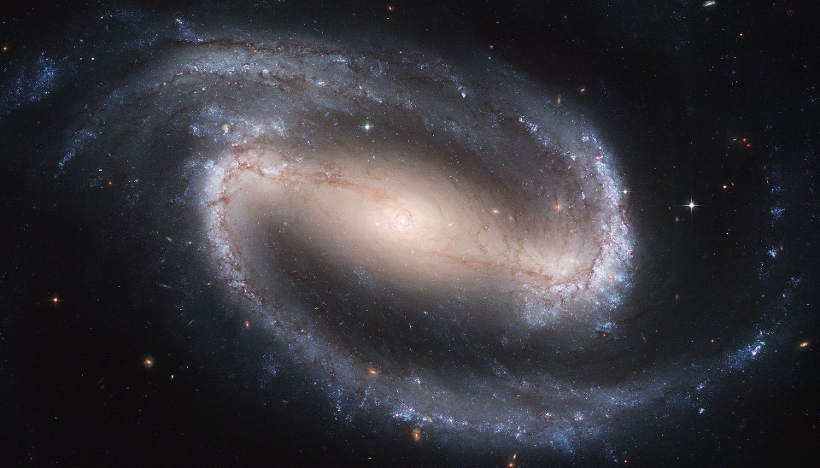
\includegraphics[width=0.85\textwidth]{figures/sampleFig1.jpg}
	\caption[Barred spiral galaxy NGC 1300]{Barred spiral galaxy NGC 1300 photographed by Hubble telescope. While the galaxy in the photo is not our sun, it does emit light, much like our sun. Image credit: NASA.}
	\label{fig:firstddd}
\end{figure}






%=======================================================%
%%%%% Do not delete this part %%%%%%
\clearpage

\printbibliography[heading=subbibintoc, title={\centering Notes}]
\end{refsection}
    
\chapter{Conclusion}
\begin{refsection}
% text of this chapter goes here


\begin{figure}[ht]
    \centering
	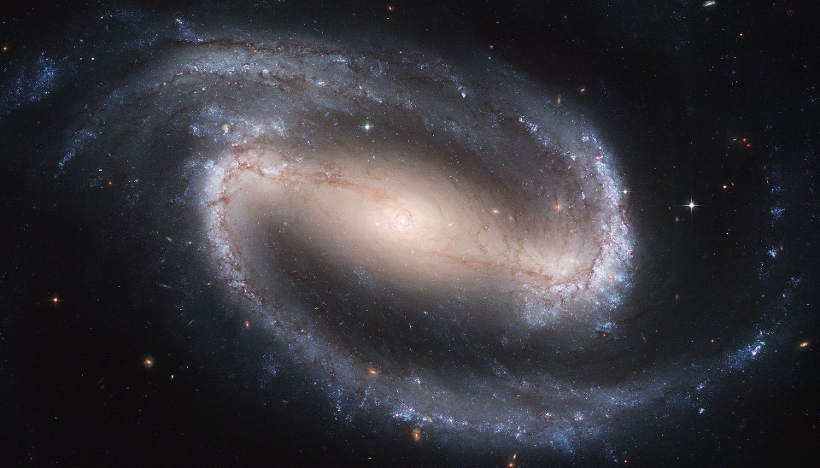
\includegraphics[width=0.85\textwidth]{figures/sampleFig1.jpg} 
	\caption[Barred spiral galaxy NGC 1300]{Barred spiral galaxy NGC 1300 photographed by Hubble telescope. While the galaxy in the photo is not our sun, it does emit light, much like our sun. Image credit: NASA.}
	\label{fig:firstFig}
\end{figure}


%=======================================================%
%%%%% Do not delete this part %%%%%%
\clearpage

\printbibliography[heading=subbibintoc, title={\centering Notes}]
\end{refsection}
    \makeBibliography
    
% The environment used here (theappendices) is a wrapper for the basic appendices environment which changes the appearance of the title page and the structure and appearance of the appendices in the table of contents and PDF bookmarks. The original functionality can be restored by simply removing the 'the' from the \begin{} and \end{} statements below.

\begin{theappendices}

\chapter{Language Editing Certification}
\centering

This is to certify that the undersigned has reviewed and went through all the pages of the Bachelor of Science in Computer Science thesis manuscript titled \\

\textbf{"FAKE NEWS DETECTION IN PHILIPPINE NEWS USING NATURAL LANGUAGE PROCESSING ALGORITHMS"} \\


of \textbf{John Louie S. Abenir}, \textbf{Jacques Nico L. Belmonte}, \textbf{Kenn Louise M. Comprado}, as against the set of structural rules that govern research writing in accord with the composition of sentences, phrases, and words in the English language.
 \newline \newline \newline \\

\noindent \textbf{JUAN DE LA CRUZ} \\
\textit{Language Editor} \\

Date:\_\_\_\_\_\_\_\_\_\_\_\_\_\_\_\_\_\_\_\_\_\_\_


\chapter{Secretary's Certification}
\centering

This is to certify that the undersigned has provided accurate recommendations, suggestions, and comments unanimously agreed and approved by the panel of examiners during the oral examination of the thesis titled \\ \textbf{"ENTER YOUR TITLE HERE"} \\  prepared and submitted by \textbf{John Louie S. Abenir}, \textbf{Jacques Nico L. Belmonte}, \textbf{Kenn Louise M. Comprado}, and that the same have not been amended, modified or obliterated. \newline \newline \newline \\



\textbf{MS. MARIA DAISY R. BELARDO} \\
\textit{Secretary} \\


Date:\_\_\_\_\_\_\_\_\_\_\_\_\_\_\_\_\_\_\_\_\_\_\_

\chapter{JOINT AFFIDAVIT OF UNDERTAKING (Plagiarism)}

\centering

\textbf{JOINT AFFIDAVIT OF UNDERTAKING}


% IN WITNESS WHEREOF, I have hereunto set my name this ____ day of ___________ 202__ in
% ___________________________________, Philippines.
% SUBSCRIBED AND SWORN TO before me this ___ day of ________ at _______________, Philippines,
% affiants exhibiting to me their competent proofs of identity above stated.
% Doc. No. ___________:
% Page No.: __________:
% Book No.: __________:
% Series of 202_.

\chapter{Source Code}

\begin{lstlisting}[language=Python, caption=Python example]
import numpy as np
    
def incmatrix(genl1,genl2):
    m = len(genl1)
    n = len(genl2)
    M = None #to become the incidence matrix
    VT = np.zeros((n*m,1), int)  #dummy variable
    
    #compute the bitwise xor matrix
    M1 = bitxormatrix(genl1)
    M2 = np.triu(bitxormatrix(genl2),1) 

    for i in range(m-1):
        for j in range(i+1, m):
            [r,c] = np.where(M2 == M1[i,j])
            for k in range(len(r)):
                VT[(i)*n + r[k]] = 1;
                VT[(i)*n + c[k]] = 1;
                VT[(j)*n + r[k]] = 1;
                VT[(j)*n + c[k]] = 1;
                
                if M is None:
                    M = np.copy(VT)
                else:
                    M = np.concatenate((M, VT), 1)
                
                VT = np.zeros((n*m,1), int)
    
    return M
\end{lstlisting}


\end{theappendices}
    % Vita should only be included for PhD candidates.

\begin{vita}

\begin{itemize}
    \item 
    
    \begin{figure}[ht]
        \centering
    	
\includegraphics[width=0.35\textwidth]{figures/person-icon.png}
    \end{figure}
    
    \textbf{J D Cruz} is a  Lorem Ipsum
    
    \item 
    
    \begin{figure}[ht]
        \centering
    	
\includegraphics[width=0.35\textwidth]{figures/person-icon.png}
    \end{figure}
    
    \textbf{J D Cruz} is a  Lorem Ipsum
    
    \item 
    
    \begin{figure}[ht]
        \centering
    	
\includegraphics[width=0.35\textwidth]{figures/person-icon.png}
    \end{figure}
    
    \textbf{J D Cruz} is a  Lorem Ipsum
\end{itemize}

\end{vita}
\end{thesisbody}

\end{document}
